\documentclass[a4paper,11pt]{kth-mag}
\usepackage[T1]{fontenc}
\usepackage{textcomp}
\usepackage{lmodern}
\usepackage[utf8]{inputenc}
\usepackage[swedish,english]{babel}
\usepackage{modifications}
\usepackage{gnuplot-lua-tikz}

\usepackage{hyperref}
\hypersetup{colorlinks,citecolor=black,filecolor=black,linkcolor=black,urlcolor=black}

\usepackage{tikz}
\usetikzlibrary{positioning}

\usepackage{clrscode3e}
\renewcommand{\gets}{\leftarrow}

\newcommand{\AND}{\land}
\newcommand{\IOR}{\lor}
\newcommand{\XOR}{\oplus}
\newcommand{\NOT}{\lnot}

\title{Using binary decision diagrams to determine program equivalence in a superoptimizer}
\subtitle{}
\foreigntitle{Att använda binära beslutsdiagram för att avgöra ekvivalens mellan program i en superoptimerare}
\author{Jesper Särnesjö}
\date{}
\blurb{Master's Thesis at CSC \\ Supervisor: Torbjörn Granlund \\ Examiner: Johan Håstad}
\trita{TRITA xxx yyyy-nn}

\begin{document}

\frontmatter

\pagestyle{empty}

\removepagenumbers

\maketitle

\selectlanguage{english}

\begin{abstract}
\end{abstract}

\clearpage

\begin{foreignabstract}{swedish}
\end{foreignabstract}

\clearpage

\tableofcontents*

\mainmatter

\pagestyle{newchap}

\chapter{Introduction}
\label{ch:introduction}

In the context of compiler technology, an \emph{optimizer} is a tool that attempts to improve the resource usage of programs.
Typically, an optimizer takes a program and transforms it using heuristics designed, for instance, to reduce execution time or memory usage.
Despite its name, however, an optimizer rarely makes a program \emph{optimal}.

A \emph{superoptimizer} takes a different approach.
Given a description of a function, it attempts to find, typically using some type of exhaustive search, the fastest or shortest program that computes that function.
In this way, a superoptimizer can generate programs that are indeed optimal.
Note, however, that due to the inefficient nature of exhaustive search, a superoptimizer can only generate very short programs, no longer than perhaps 5 or 6 instructions, in reasonable time.
Further, a superoptimizer can only generate \emph{straight-line} programs, that is, programs that contain no loops, branches or other jumps.
Despite this, superoptimizers can be useful for optimizing inner loops and other small sequences of code required to be fast or small.

A crucial capability of a superoptimizers, is the ability to determine if a found program and the input function are \emph{equivalent}, meaning that they always yield identical output given identical and valid input.
This thesis explores using \emph{binary decision diagrams} (BDDs), data structures capable of efficiently representing Boolean functions, for this purpose.

% overview of thesis

Chapter~\ref{ch:background}

Chapter~\ref{ch:target_architecture}

Chapter~\ref{ch:design_implementation}

% note on Boolean notation?

\chapter{Background}
\label{ch:background}

\section{Superoptimizers}

\subsection{Massalin's superoptimizer}

The term \emph{superoptimizer} was coined by Massalin in a 1987 paper \cite{massalin87}, to describe a tool for finding the shortest straight-line program that computes a given function.

Massalin's implementation takes as its input a program written in assembly language for the Motorola 68020 processor.
It then consults a table containing a subset of the processor's instruction set, and begins generating all combinations of these instructions, beginning with those of length 1, then 2, and so on.
Each generated program is tested for equivalence with the input program.
When a program passes the test, it is printed, and the search terminates.
Because programs are tested in order of increasing length, this program will necessarily be \emph{optimal} in terms of length, meaning that no shorter equivalent program exists.

Naturally, exhaustively searching the space of all possible programs is a very inefficient process, considering that the number of programs of length $n$ is $b^n$, where $b$ is the \emph{branching factor} of the search tree.
To find a value of $b$, consider an architecture with $r$ registers, and an instruction set consisting of $i_0$ instructions that take no arguments, $i_1$ instructions that take one argument, and $i_2$ instructions that take two arguments.
For this architecture, the branching factor would be, in the worst case, $i_0+i_1r+i_2r^2$.
Even for modest values of $i_0$, $i_1$, $i_2$ and $r$, the branching factor would end up in the hundreds or thousands.
Hence, a naive superoptimizer is only capable of generating very short programs in reasonable time.

To address this, Massalin describes a method of \emph{pruning} the search tree.
Using this method, the superoptimizer keeps a lookup table, where short instruction sequences known to be non-optimal are marked as such.
When a program is found to contain a non-optimal instruction sequence, it is rejected without being tested.

Massalin also describes two methods of determining whether a candidate program is equivalent to the input program.

The first method, referred to as the \emph{Boolean test}, is to express both programs in Boolean logic, reduce them to an unspecified canonical form, and compare them minterm for minterm.
Using this method, Massalin's superoptimizer is capable of testing 40 programs of an unspecified length per second, when running on a 16 MHz processor.

The second method, referred to as the \emph{probabilistic test}, is to simply execute both programs with identical input, and compare their output.
This method is significantly faster, allowing the superoptimizer to test 50000 programs per second.
However, it introduces the risk of false positives, in the form of programs that are equivalent only on the input used, not in the general case.
Hence, manual verification of the output is required.
Further, whereas the Boolean test can be used on any kind of program, Massalin's probabilistic test can only be used on programs written in the assembly language of the host architecture.

It is worth noting, that even with such a significant increase in speed, only slightly longer programs may be generated in reasonable time with a realistic branching factor, as illustrated by Figure~\ref{fig:so_program_length}.

% stress this

\begin{figure}
\centering
\include{so_program_length}
\caption{The maximum length of a program generated in 24 hours, as a function of the branching factor.
The solid and dashed lines represent Massalin's superoptimizer using the Boolean and probabilistic tests, respectively.}
\label{fig:so_program_length}
\end{figure}

\subsection{GSO}

GSO, the GNU superoptimizer, is described in a 1992 paper by Granlund and Kenner \cite{granlund92}.

Like Massalin's superoptimizer, GSO optimizes for program length.
It uses a probabilistic equivalence test, and as such its output must be manually verified.
Unlike the probabilistic test in Massalin's superoptimizer, which executes instructions directly on the host architecture, GSO's test \emph{simulates} them using functions that operate on a virtual machine of sorts, consisting of a set of registers and a single carry bit.
GSO is therefore capable of supporting a wide range of architectures, but also requires that the input program be specified as a compiled-in \emph{goal function}.

Granlund and Kenner also describe numerous methods of pruning used in GSO.
When selecting arguments for generated instructions, GSO only considers live registers, that is, registers that contain input values or have previously been written to.
Similarly, instructions that read the carry flag are only generated after it has been set.
For commutative instructions, that is, instructions for which arguments can be ordered in different ways without changing the meaning of the instruction, only one argument ordering is tried.

When generating the last instruction in a program, GSO is even more restrictive.
Specifically, it requires that the last instruction reads a register or the carry flag written to by the preceding instruction, since that instruction would otherwise be superfluous.

\subsection{Denali}

Denali is a superoptimizer created by Joshi et al, then at Compaq Systems Research Center, first described in a 2002 paper \cite{joshi02}.

Denali's design differs greatly from that of Massalin's superoptimizer and GSO.
Rather than generating programs and then testing them, Denali starts by generating a set of programs equivalent to the input program, and then selects the optimal among them.

To accomplish the first step, Denali requires a set of \emph{axioms}, which describe how instructions may be substituted for another without changing the meaning of the program.
Such axioms may, for example, state that multiplication by $2^n$ is the same as right-shift by $n$.
Axioms are also used to mark instructions as commutative or associative, and to specify their identity, for instance 0 for addition and 1 for multiplication.

To select the optimal program, Denali rewrites the problem as a satisfiability problem, which is handed off to an external SAT solver.

The authors claim that Denali is capable of optimizing for \emph{execution time}, that is, the number of cycles required for the program to terminate.
This is remarkable, as determining the execution time for a program is more complicated than it may seem.
The number of cycles required to execute an instruction, depends not only on the instruction itself, but also possibly on the instructions surrounding it, due to pipelining.
In a follow-up paper \cite{joshi06}, the authors describe a simplified design, named Denali-2, which instead optimizes for program length.

% input in somewhat C-like DSL
% multiple assignments
% Alpha EV-6

\subsection{Bansal's superoptimizer}

The superoptimizer created by Bansal and described in his 2008 PhD thesis \cite{bansal_thesis} differs from the ones described above, in that it requires no human supervision, neither for verifying its output, nor for selecting its input.
Instead, it reads binaries compiled for the x86 architecture, harvesting instruction sequences to optimize.
Its output is not an optimized program, but rather the optimizations discovered.
In this way, Bansal's superoptimizer is capable of autonomously generating a very large library of optimizations, which can then be used by an ordinary peephole optimizer.

Since output is required to be correct, optimizations are verified by a Boolean test performed by a SAT solver.
To improve speed, candidate optimizations are first screened by a probabilistic test similar to that found in Massalin's superoptimizer and GSO.

% no numbers given?

Other notable features of Bansal's superoptimizer is that it is capable of optimizing both for execution time and for program size, and that it utilizes a meet-in-the-middle method of pruning.
Using this method, the superoptimizer searches not only \emph{forwards} for progressively longer programs, but also \emph{backwards} from the state the architecture is required to be in following correct program execution.

\subsection{TOAST}

TOAST, short for \emph{total optimisation using answer set technology}, is a superoptimizer created by Crick and described in his 2009 PhD thesis \cite{crick_thesis}.
It is implemented using Answer Set Programming, a declarative logic programming language.
Like Denali and Bansal's superoptimizer, it produces provably correct output.

%\subsection{...}
%
%\cite{aha}
%\cite{pic}

\section{Binary decision diagrams}
\label{s:bdds}

\emph{Binary decision diagrams} (BDDs) are data structures used to represent Boolean functions.
They consist of nodes, representing the function's variables. Each node has one or more incoming paths, and exactly two outgoing paths, commonly referred to as the \emph{high} and \emph{low} path.
When using a BDD to determine the value of a Boolean function, one follows a node's high path if its variable is 1, and its low path if its variable is 0, starting at the root node, until one arrives at a terminal node.

There are many types of BDDs, of which some can be used to store and manipulate Boolean functions very efficiently.
However, the performance of the operations performed on a BDD, varies greatly depending on the function represented, and the order in which its variables are indexed.

BDDs were introduced by Lee \cite{lee59}, under the name \emph{binary-decision programs}.
They were given their current name by Akers \cite{akers78}, who also explored the ideas of \emph{reducing} BDDs by removing redundant nodes, and of representing multiple functions in a single BDD.

A more restricted type of BDD was introduced by Bryant \cite{bryant86}.
In addition to the above, Bryant required the BDD to be \emph{ordered}, having its variables appear in the same order on all paths from the root to a terminal node,
and to be \emph{reduced}, containing no node with the same high and low path, and no two distinct nodes with isomorphic subgraphs.
Such a BDD is called a \emph{reduced ordered BDD} (ROBDD), and has several beneficial characteristics.
First, the algorithms used to perform Boolean operations on one or a pair of ROBDDs, are efficient, requiring at worst a number of time steps proportional to the product of the number of nodes in the two ROBDDs.
Further, ROBDDs are \emph{canonical} representations of their Boolean functions, meaning that two Boolean functions are equivalent iff their ROBDDs are isomorphic.

Bryant also further explored the idea of representing multiple functions in a single BDD, which would later be referred to as a \emph{shared BDD} by Minato et al \cite{minato90}.

A BDD with all these characteristics, a \emph{shared reduced ordered BDD} (SROBDD), has the added benefits of being memory efficient, and of allowing an isomorphism test to be implemented as a single pointer comparison.

Bryant showed that the variable ordering used can have a dramatic effect on the number of nodes in a BDD, which in the best case is linear in the number of variables, and in the worst case exponential.
Bryant states that finding the variable ordering that minimizes the number of nodes is an NP-complete problem.
Bollig and Wegener \cite{bollig96} would later show that even determining whether an ordering exists for which the number of nodes is at most a given value, is an NP-complete problem.

Bryant asserts that for many functions, a good variable ordering can be determined by examining the structure of the functions.
As an example, he mentions that for functions in which variables primarily interact pairwise, ordering variables and their partners consecutively gives good results.

However, Bryant also states that there are functions that can only be represented using a number of nodes exponential in the number of variables, regardless of variable ordering, and proves that integer multiplication is such a function.

% lower bounds given by Bollig and Wegener

\subsection{Example}

To illustrate how a moderately complex Boolean function can be represented by a BDD, consider an adder that takes two $n$-bit numbers, $a$ and $b$, and produces their sum, as well a carry-out bit.

To express the adder in Boolean logic, we represent $a$ as $n$ Boolean variables $\langle a_0, a_1, ..., a_{n-1} \rangle$, where $a_0$ and $a_{n-1}$ are the least and most significant bits of $a$, respectively.
Doing the same for $b$, we get a total of $2n$ variables.

The function for the carry-out bit, $c_{n-1}$, depends on every variable, and can be defined recursively as follows:

$$
  c_k = \left\{
  \begin{array}{ll}
    a_k \AND b_k                                             & k = 0 \\
    a_k \AND b_k \IOR a_k \AND c_{k-1} \IOR b_k \AND c_{k-1} & 0 < k < n \\
  \end{array}\right.
$$

For $n = 2$, $c_1$ can be represented as the truth table shown in Table~\ref{tab:tt_c1}, or, using the variable ordering $a_0,b_0,...,a_{n-1},b_{n-1}$, as an OBDD or ROBDD as shown in Figure~\ref{fig:bdd_c1}.
Note that the ROBDD representation is quite compact, and that not all variables are present on every path.
For instance, if $a_0$ is 0, there is no need to check $b_0$, and we instead skip ahead to $a_1$.

Not all variable orderings produce such compact ROBDDs for this function, however.
If we instead use the variable ordering $a_0,...,a_{n-1},b_0,...,b_{n-1}$, we end up with a larger ROBDD.
This becomes more clear for larger values of $n$, as illustrated in Figure~\ref{fig:bdd_c2_bad}.

Upon inspection, we find that in the ROBDD representation of this particular function, using these two variable orderings, the number of nodes is:

$$
  |c_{n-1}| = \left\{
  \begin{array}{ll}
    3n-1      & \textrm{using variable order $a_0,b_0,...,a_{n-1},b_{n-1}$} \\
    2^{n+1}-2 & \textrm{using variable order $a_0,...,a_{n-1},b_0,...,b_{n-1}$} \\
  \end{array}\right.
$$

For $n = 32$, the ROBDD would consequently contain only 97 nodes with the first variable ordering, but over 8 billion with the second.

Note that Bryant's suggested method of ordering interacting variables consecutively, works very well in this case.

\begin{table}
\centering
\begin{tabular}{cccc|cc}
$a_0$ & $b_0$ & $a_1$ & $b_1$ & $c_0$ & $c_1$ \\
\hline
0     & 0     & 0     & 0     & 0     & 0 \\
0     & 0     & 0     & 1     & 0     & 0 \\
0     & 0     & 1     & 0     & 0     & 0 \\
0     & 0     & 1     & 1     & 0     & 1 \\
0     & 1     & 0     & 0     & 0     & 0 \\
0     & 1     & 0     & 1     & 0     & 0 \\
0     & 1     & 1     & 0     & 0     & 0 \\
0     & 1     & 1     & 1     & 0     & 1 \\
1     & 0     & 0     & 0     & 0     & 0 \\
1     & 0     & 0     & 1     & 0     & 0 \\
1     & 0     & 1     & 0     & 0     & 0 \\
1     & 0     & 1     & 1     & 0     & 1 \\
1     & 1     & 0     & 0     & 1     & 0 \\
1     & 1     & 0     & 1     & 1     & 1 \\
1     & 1     & 1     & 0     & 1     & 1 \\
1     & 1     & 1     & 1     & 1     & 1 \\
\end{tabular}
\caption{Truth table for the Boolean function $c_1$.}
\label{tab:tt_c1}
\end{table}

\begin{figure}[p]
\centering
\include{bdd_c1}
\caption{The Boolean function $c_1$ as an OBDD (left) and an ROBDD (right). The solid lines represent high paths and the dashed lines represent low paths.}
\label{fig:bdd_c1}
\end{figure}

\begin{figure}[p]
\centering
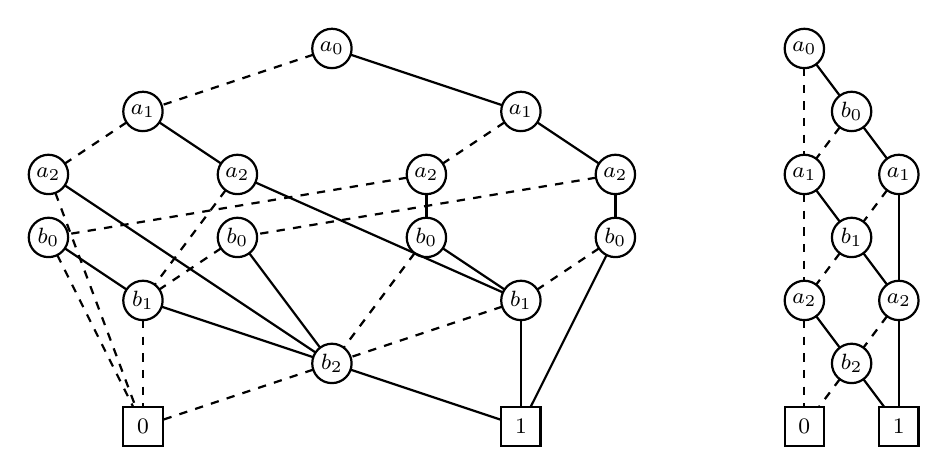
\begin{tikzpicture}
[every node/.style={draw=black,thick,minimum size=5mm,inner sep=0mm,outer sep=0mm,font=\footnotesize},
 var/.style={circle},
 val/.style={rectangle},
 thick]
\node[var] (a0)                                            {$a_0$};
\node[var] (a1A) [on grid,below  left=8mm and 24mm of a0]  {$a_1$};
\node[var] (a1B) [on grid,below right=8mm and 24mm of a0]  {$a_1$};
\node[var] (a2A) [on grid,below  left=8mm and 12mm of a1A] {$a_2$};
\node[var] (a2B) [on grid,below right=8mm and 12mm of a1A] {$a_2$};
\node[var] (a2C) [on grid,below  left=8mm and 12mm of a1B] {$a_2$};
\node[var] (a2D) [on grid,below right=8mm and 12mm of a1B] {$a_2$};
\node[var] (b0A) [on grid,below right=8mm and  0mm of a2A] {$b_0$};
\node[var] (b0B) [on grid,below right=8mm and  0mm of a2B] {$b_0$};
\node[var] (b0C) [on grid,below right=8mm and  0mm of a2C] {$b_0$};
\node[var] (b0D) [on grid,below right=8mm and  0mm of a2D] {$b_0$};
\node[var] (b1A) [on grid,below right=8mm and 12mm of b0A] {$b_1$};
\node[var] (b1B) [on grid,below right=8mm and 12mm of b0C] {$b_1$};
\node[var] (b2)  [on grid,below right=8mm and 24mm of b1A] {$b_2$};
\node[val] (0)   [on grid,below  left=8mm and 24mm of b2]  {0};
\node[val] (1)   [on grid,below right=8mm and 24mm of b2]  {1};
\path[dashed] (a0)  edge (a1A);
\path         (a0)  edge (a1B);
\path[dashed] (a1A) edge (a2A);
\path         (a1A) edge (a2B);
\path[dashed] (a1B) edge (a2C);
\path         (a1B) edge (a2D);
\path[dashed] (a2A) edge (0);
\path         (a2A) edge (b2);
\path[dashed] (a2B) edge (b1A);
\path         (a2B) edge (b1B);
\path[dashed] (a2C) edge (b0A);
\path         (a2C) edge (b0C);
\path[dashed] (a2D) edge (b0B);
\path         (a2D) edge (b0D);
\path[dashed] (b0A) edge (0);
\path         (b0A) edge (b1A);
\path[dashed] (b0B) edge (b1A);
\path         (b0B) edge (b2);
\path[dashed] (b0C) edge (b2);
\path         (b0C) edge (b1B);
\path[dashed] (b0D) edge (b1B);
\path         (b0D) edge (1);
\path[dashed] (b1A) edge (0);
\path         (b1A) edge (b2);
\path[dashed] (b1B) edge (b2);
\path         (b1B) edge (1);
\path[dashed] (b2)  edge (0);
\path         (b2)  edge (1);
\node[var] (Ga0)  [on grid,right=60mm of a0]                {$a_0$};
\node[var] (Gb0)  [on grid,below right=8mm and 6mm of Ga0]  {$b_0$};
\node[var] (Ga1A) [on grid,below  left=8mm and 6mm of Gb0]  {$a_1$};
\node[var] (Ga1B) [on grid,below right=8mm and 6mm of Gb0]  {$a_1$};
\node[var] (Gb1)  [on grid,below right=8mm and 6mm of Ga1A] {$b_1$};
\node[var] (Ga2A) [on grid,below  left=8mm and 6mm of Gb1]  {$a_2$};
\node[var] (Ga2B) [on grid,below right=8mm and 6mm of Gb1]  {$a_2$};
\node[var] (Gb2)  [on grid,below right=8mm and 6mm of Ga2A] {$b_2$};
\node[val] (G0)   [on grid,below  left=8mm and 6mm of Gb2]  {0};
\node[val] (G1)   [on grid,below right=8mm and 6mm of Gb2]  {1};
\path[dashed] (Ga0)  edge (Ga1A);
\path         (Ga0)  edge (Gb0);
\path[dashed] (Gb0)  edge (Ga1A);
\path         (Gb0)  edge (Ga1B);
\path[dashed] (Ga1A) edge (Ga2A);
\path         (Ga1A) edge (Gb1);
\path[dashed] (Ga1B) edge (Gb1);
\path         (Ga1B) edge (Ga2B);
\path[dashed] (Gb1)  edge (Ga2A);
\path         (Gb1)  edge (Ga2B);
\path[dashed] (Ga2A) edge (G0);
\path         (Ga2A) edge (Gb2);
\path[dashed] (Ga2B) edge (Gb2);
\path         (Ga2B) edge (G1);
\path[dashed] (Gb2)  edge (G0);
\path         (Gb2)  edge (G1);
\end{tikzpicture}

\caption{The Boolean function $c_2$ in ROBDD form using the variable order $a_0,a_1,a_2,b_0,b_1,b_2$ (left) and $a_0,b_0,a_1,b_1,a_2,b_2$ (right).}
\label{fig:bdd_c2_bad}
\end{figure}

\chapter{Target architecture}
\label{ch:target_architecture}

The superoptimizer implemented as part of this thesis project targets the x86 architecture, as described by the manuals published by Intel Corporation \cite{intel_1,intel_2a,intel_2b}.

Since the x86 architecture is large and quite complex, it should be stressed that the superoptimizer only supports a very small subset of its features.
While there are hundreds of instructions in the x86 general purpose instruction set, and many more in its numerous extensions, the superoptimizer's instruction set contains only 33 instructions.
These instructions operate only on registers and flags, passing in immediate values or addressing the memory is not supported.

% all registers same size, not all flags

The assembly language used to describe programs accepted as input or produced as output by the superoptimizer is similar, but not identical, to the one used by Intel.
Programs generated by the superoptimizer can, with minor syntactical modifications, be assembled and executed on a real x86 machine.

% this chapter describes architecture in brief and to aid understanding of superoptimizer operation
% not intended as programming guide nor complete description
% complete and in-depth information can be found in Intel's manuals.

\section{Registers}

Registers are used to hold integer values, and are read from and written to by instructions.
Two's-complement arithmetic is used to represent negative numbers, but since registers are typeless, whether a given register contains a signed or an unsigned integer is determined solely by how it is used.
Indeed, registers do not have to represent integers, but can be seen simply as sets of bits.

There are 8 registers in the superoptimizer's architecture, each 32 bits in size.

\section{Flags}
\label{s:flags}

Flags are single-bit values used to signify various conditions.
They are written to and read from by instructions, in general as a side effect rather than directly.

There are 17 different flags in the x86 architecture, but the superoptimizer only supports the 5 for which a corresponding \verb|cmov| instruction exists:
the \emph{carry} (\verb|cf|), \emph{overflow} (\verb|of|), \emph{parity} (\verb|pf|), \emph{sign} (\verb|sf|) and \emph{zero} (\verb|zf|) flags.

\verb|cf| and \verb|of| are used to signify that overflow has occured, meaning that the result of an operation did not fit into a single register.
\verb|cf| is used for unsigned arithmetic, while \verb|of| is used for signed arithmetic, but their exact meaning varies from instruction to instruction.

\verb|pf|, \verb|sf| and \verb|zf| can be determined entirely by inspecting the result of an operation.
\verb|pf| signifies that that an even number of the least significant 8 bits in the result are set to 1,
\verb|sf| that the result is negative if interpreted as a signed number, since the most significant bit is 1,
and \verb|zf| that every bit is 0.

\section{Language}
\label{s:language}

Programs accepted as input or produced as output by the superoptimizer, use Intel's syntax with a few modifications.
Registers are referred to as \verb|r0|, \verb|r1|, and so on, rather than the usual names \verb|eax|, \verb|ebx|, etc.
Statements are terminated by semicolons rather than newlines.

If an instruction takes arguments, the first one specifies the \emph{destination} register, which may be read from, written to, or both.
If an instruction takes two arguments, the second one specifies the \emph{source} register, which is only read from.

As an example, a program that sets \verb|r0| to the sum of \verb|r1| and \verb|r2|, could be written as follows:

\begin{verbatim}
mov r0,r1; add r0,r2;
\end{verbatim}

\section{Instruction set}

% discuss how to select insn set
% only include worthwhile insns
% keep insn count low = keep branching factor low
% also, by not including slow insns, program-length optimal -> reasonably execution-time "optimal"
% slow measured by latency, throughput
\cite{x86_timing}

% different i/o insn sets

% however, for this thesis, insns chosen for variety and to highlight strengths and weaknesses of BDD test

The supported instructions are listed in Table~\ref{tab:insns}, which also gives an overview of their behavior with regards to the destination and source registers, as well as flags.

\begin{table}
\centering
\begin{tabular}{l|cc|ccccc}
instruction   & d  & s  & \verb|cf| & \verb|of| & \verb|pf| & \verb|sf| & \verb|zf| \\
\hline
\verb|stc|    &    &    & W         &           &           &           &           \\
\verb|clc|    &    &    & W         &           &           &           &           \\
\verb|cmc|    &    &    & RW        &           &           &           &           \\
\hline
\verb|mov|    & W  & R  &           &           &           &           &           \\
\verb|cmovc|  & RW & R  & R         &           &           &           &           \\
\verb|cmovo|  & RW & R  &           & R         &           &           &           \\
\verb|cmovp|  & RW & R  &           &           & R         &           &           \\
\verb|cmovs|  & RW & R  &           &           &           & R         &           \\
\verb|cmovz|  & RW & R  &           &           &           &           & R         \\
\verb|cmovnc| & RW & R  & R         &           &           &           &           \\
\verb|cmovno| & RW & R  &           & R         &           &           &           \\
\verb|cmovnp| & RW & R  &           &           & R         &           &           \\
\verb|cmovns| & RW & R  &           &           &           & R         &           \\
\verb|cmovnz| & RW & R  &           &           &           &           & R         \\
\verb|cmova|  & RW & R  & R         &           &           &           & R         \\
\verb|cmovbe| & RW & R  & R         &           &           &           & R         \\
\verb|cmovg|  & RW & R  &           & R         &           & R         & R         \\
\verb|cmovge| & RW & R  &           & R         &           & R         &           \\
\verb|cmovl|  & RW & R  &           & R         &           & R         &           \\
\verb|cmovle| & RW & R  &           & R         &           & R         & R         \\
\hline
\verb|and|    & RW & R  & W         & W         & W         & W         & W         \\
\verb|or|     & RW & R  & W         & W         & W         & W         & W         \\
\verb|xor|    & RW & R  & W         & W         & W         & W         & W         \\
\verb|not|    & RW &    &           &           &           &           &           \\
\hline
\verb|add|    & RW & R  & W         & W         & W         & W         & W         \\
\verb|adc|    & RW & R  & RW        & W         & W         & W         & W         \\
\verb|sub|    & RW & R  & W         & W         & W         & W         & W         \\
\verb|sbb|    & RW & R  & RW        & W         & W         & W         & W         \\
\verb|cmp|    & R  & R  & W         & W         & W         & W         & W         \\
\verb|inc|    & RW &    &           & W         & W         & W         & W         \\
\verb|dec|    & RW &    &           & W         & W         & W         & W         \\
\verb|neg|    & RW &    & W         & W         & W         & W         & W         \\
\hline
\verb|imul|   & RW & R  & W         & W         & -         & -         & -         \\
\end{tabular}
\caption{The instruction set of the superoptimizer.} % explain d/s, R/W/-
\label{tab:insns}
\end{table}

\subsection{Flag control}

The simplest supported instructions are the flag control instructions.
\verb|stc| and \verb|clc| set \verb|cf| to 1 and 0, respectively.
\verb|cmc| complements \verb|cf|, flipping it from 0 to 1 or vice versa.
These instructions do not modify registers in any way.

\subsection{Data transfer}

The data transfer instructions copy the value of a source register to a destination register.
\verb|mov| does so unconditionally, while the \verb|cmov| family of instructions does so only if a given condition is true, otherwise leaving the destination register unmodified.

There are 30 \verb|cmov| instructions in the x86 instruction set, but many of these are duplicates, presumably created to allow assembly language programmers to more clearly express their intent.
The superoptimizer only supports the 16 instructions with unique behavior.

\verb|cmovc|, \verb|cmovo|, \verb|cmovp|, \verb|cmovs| and \verb|cmovz|, as well as \verb|cmovnc|, \verb|cmovno|, \verb|cmovnp|, \verb|cmovns| and \verb|cmovnz|, only inspect the value of a single flag, transferring data if that flag is set to an expected value.

\verb|cmova|, \verb|cmovbe|, \verb|cmovg|, \verb|cmovge|, \verb|cmovl| and \verb|cmovle|, on the other hand, inspect the values of several flags.
They can be placed following \verb|cmp| or another instruction that sets flags by comparing two values, in order to transfer data if one value is, for instance, greater or less than another.

% above/below for unsigned
% greater/less for signed

% cmovc/cmovb/cmovnae  carry/below/not above or equal
% cmovo                overflow
% cmovp/cmovpe         parity/parity even
% cmovs                sign
% cmovz/cmove          zero/equal
% cmovnc/cmovae/cmovnb not carry/above or equal/not below
% cmovno               not overflow
% cmovnp/cmovpo        not parity/parity odd
% cmovns               not sign
% cmovnz/cmovne        not zero/not equal
% cmova/cmovnbe        above/not below or equal
% cmovbe/cmovna        below or equal/not above
% cmovg/cmovnle        greater/not less or equal
% cmovge/cmovnl        greater or equal/not less
% cmovl/cmovnge        less/not greater or equal
% cmovle/cmovng        less or equal/not greater

As shown in Table~\ref{tab:insns}, \verb|mov| is considered to read from one register and write to another, while the \verb|cmov| instructions are considered to read from both, and write to one.
This, together with a requirement that instructions only read from registers with defined values, ensures that the value of the destination register remains well-defined.

The data transfer instructions do not modify any flags.

\subsection{Logic}

The instruction set contains four instructions that perform bitwise Boolean logic.

\verb|and|, \verb|or| and \verb|xor| all take two arguments, and perform bitwise logical \emph{and}, \emph{inclusive-or} and \emph{exclusive-or}, respectively.
These instructions always set \verb|cf| and \verb|of| to 0, while \verb|pf|, \verb|sf| and \verb|zf| are set based on the result as described in Section~\ref{s:flags}.

\verb|not| takes a single argument and performs bitwise logical negation on it.
It does not modify any flags.

\subsection{Addition and subtraction}

A large number of the supported instructions perform some variant of addition or subtraction.

The most basic of these is \verb|add|, which takes two arguments and performs integer addition on them.
Since two's-complement arithmetic is used, \verb|add| performs both signed and unsigned addition simultaneously, with \verb|cf| and \verb|of| set to indicate unsigned and signed overflow, respectively.
\verb|pf|, \verb|sf| and \verb|zf| are set based on the result as described in Section~\ref{s:flags}.

\verb|adc| performs addition with \emph{carry-in}, meaning that it adds not only its two arguments, but also \verb|cf|.

\verb|sub| and \verb|sbb| are the subtraction counterparts of \verb|add| and \verb|adc|.
\verb|cmp| behaves the same as \verb|sub| with regards to flags, but does not write its result to a register.

\verb|inc| and \verb|dec| behave like \verb|add| and \verb|sub|, but take only one argument, substituting the value 1 for the second argument.
They do not alter the value of \verb|cf|, but modify the other flags in the same way as \verb|add|.

\verb|neg| takes one arguments and performs two's-complement negation on it.
It sets \verb|cf| to 0 if its argument is 0, and 1 otherwise, and modifies the other flags in the same way as \verb|add|.

\subsection{Multiplication}

The x86 instruction set contains many multiplication instructions, each with slightly different behavior.
The only instruction supported by the superoptimizer is the form of \verb|imul| that takes two arguments and performs integer multiplication on them, truncating the result to fit into a single register.

\verb|cf| and \verb|of| are both used to indicate that the truncated result differs from the actual result, meaning that overflow has occured.
\verb|pf|, \verb|sf| and \verb|zf|, however, are left in an \emph{undefined} state.

\chapter{Design and implementation}
\label{ch:design_implementation}

The superoptimizer implemented as part of this thesis project takes a program written in the assembly language described in Section~\ref{s:language} as its input.
It then begins generating candidate programs, testing them for equivalence with the input program.
Programs are generated in order of increasing length, meaning that the first program to be printed will be optimal in terms of length.
The superoptimizer continues generating and testing programs until it reaches a user-specified maximum length, or is terminated by the user.

% design primarily inspired by GSO?

The superoptimizer was implemented using C and C++.
A suite of unit tests was created to aid development, but no formal verification of correctness was performed.

\section{Determining register usage}

% initial step
% used by generator, tests

The programs supported by the superoptimizer have any number of input registers, and a single output register.

Input registers are assumed to contain well-defined values at the start of the program's execution.
Programs generated by the superoptimizer are allowed, but not required, to read from these registers.

The output register is considered to contain the return value of the entire program.
Generated programs are required to use the same output register as the input program.
Indeed, the superoptimizer determines equivalence based solely on the output register, ignoring the values of all other registers and the flags.

To determine the input and output registers of the input program, the superoptimizer steps through its instructions in order, marking any register that is read from before it is written to as an input register, and the last register written to as the output register.

\section{Generating candidate programs}

The superoptimizer uses an iterative deepening depth-first search to find programs equivalent to the input programs.
Initially, the depth limit is 1, meaning that programs of of length 1 are generated.
Once all programs of length 1 have been tested or pruned, the depth limit is increased to 2, and so on.
This continues until a user-specified maximum length has been reached, or the superoptimizer is terminated by the user.

% neither 0-length programs nor nop supported, xo can't optimize 'and r0,r0;'

The superoptimizer prunes the search tree by not generating some types of programs which cannot possibly be equivalent to the input program.

In particular, the superoptimizer does not generate programs that read from registers or flags whose values are not well-defined. % explain why?
For this, the superoptimizer keeps a \emph{live set} of registers, which initially consists of the input registers, as well as one of flags, which initially is empty.
When selecting registers for instructions, only those is the live set are considered.
Similarly, instructions that read flags are only generated if those flags are in the live set.
After generating an instruction that writes to a register or flags, the superoptimizer adds that register or those flags to their respective live sets.
% registers never removed from live set
% flags can be (imul)

% in addition, some instructions are special-cased:

\verb|xor| and \verb|sub| can both be used to set a register to 0, by using that register both as the destination and source register.
Similarly, \verb|sbb| can be used to set a register to \verb|-cf|.
Since this does not depend on the register's previous value, the registers used by these instructions need not be in the live set.

For \verb|mov| and \verb|cmov| instructions, the destination register is required to be different from the source register, since the instruction would otherwise be superfluous.
For \verb|mov|, the destination register is also required to be the output register of the program, or a register \emph{not} in the live set.

The last instruction in a program is required to write to the output register.
% note! does not use GSO pruning that last insn must read reg or flag written to by preceding insn

Once an entire program has been generated, it is tested for equivalence with the input program as described below.
Programs found to be equivalent to the input program are printed.

% as a note, the code for the program generator grew quite messy over time, and that it is likely that it contains some bugs.

\section{Testing for equivalence with input program} % or: determining equivalence?

% BDD or Boolean?

The superoptimizer tests each generated candidate program for equivalence with the input program using a probabilistic test and a test based on BDDs.
The probabilistic test is fast, but may report false positives, while the BDD test is slow but correct, barring any bugs in its implementation.
For this reason, the probabilistic test is run first, eliminating most non-equivalent programs, with the BDD test applied only to programs that pass the probabilistic test.

The probabilistic and BDD tests can be seen as two independent implementations of the architecture defined in Chapter~\ref{ch:target_architecture}.
If should be noted, however, that neither of them are capable of correctly handling programs which read from undefined registers or flags, since such programs are not expected to be generated.

\subsection{Probabilistic test}

The superoptimizer uses a probabilistic test similar to the one used by GSO.
It's implementation, written in C, represents registers by unsigned integers, flags by single bits, and instructions by functions.
Since the instructions were generally simple enough to be implemented using a single C operator, they will not be described in further detail.

When comparing a candidate program for equivalence to the input program, two sets of registers and flags are used.
In both, the registers are set to values taken from a hardcoded test vector, and the flags are set to 0.
Initially, the two sets are identical.

The functions representing the input program's instructions are then run in order on one of the sets, while those representing the candidate program are run on the other.
The output registers are then compared.
If they differ, the programs are not equivalent, and the test end.
If they are equal, the test starts over, using new values taken from the test vector.
If all values in the test vector have been used, the candidate program passes the test, as it is equivalent to the input program at least for the values used.

Since it is possible that the candidate program is in fact not equivalent to the input program for some values not used, one might ask why the programs are not tested using \emph{all} possible values.
Indeed, for a program with a single 32-bit input register, there are only $2^{32}$ possible values to test.
Considering that programs generated by a superoptimizer are no longer than 5 or 6 instructions, running them $2^{32}$ times should take less than a minute on a modern computer.

However, this method will not work well even for programs with two input registers.
Such a program would need to be run $2^{64}$ times, which would take several thousand years.

% (2^32 * 5 * 3) / (2 GHz) = 32 seconds
% (2^64 * 5 * 3) / (2 GHz) = 4384 years

Hence, programs are tested using only a few hardcoded values, with equivalence being determined definitively by the BDD test.

\subsection{BDD test}

To determine if two programs are equivalent, one can translate both into Boolean logic, reduce them to some canonical form, and compare them.
The superoptimizer uses BDDs, or more specifically SROBDDs, as described in Section~\ref{s:bdds}, for this purpose.

The implementation was written in C++, using the software package BuDDy \cite{buddy}.
BuDDy was chosen out of a small pool of alternatives, for its reasonably well-written documentation and apparent popularity.
No formal evaluation of alternatives was performed.

\subsubsection{Overview}

Each bit in each register is represented by a reference to an SROBDD, as is each flag.
Initially, the registers reference variables, while the flags all reference the constant 0.

When translating a program to SROBDD form, the superoptimizer steps through its instructions in order.
For each instruction, the references in its outputs are set to SROBDDs that are functions of its inputs.
Crucially, once the superoptimizer has stepped through all instructions, the output register will be represented by 32 SROBDDs, which are functions of the initial variables.

To determine if a candidate program is equivalent to the input program, the superoptimizer translates both to SROBDD form, and compares the SROBDDs representing their output registers pairwise.
If all are equal, the two programs are equivalent.

In the descriptions below, a register $a$ is represented by 32 Boolean variables $\langle a_0, a_1, ..., a_{n-1} \rangle$, where $a_0$ and $a_{n-1}$ are the least and most significant bits of $a$, respectively.
The flags are represented as $f_c$, $f_o$, $f_p$, $f_s$ and $f_z$.
An instruction \verb|foo| is represented by a pseudocode function \proc{foo}.

\subsubsection{Flags}

The instructions that set $f_p$, $f_s$ or $f_z$, all do so in the same way.
With $a$ as the result register, these flags are set as follows:

\begin{codebox}
\zi $f_p \gets \NOT(a_0 \XOR a_1 \XOR ... \XOR a_7)$
\zi $f_s \gets a_{n-1}$
\zi $f_z \gets \NOT(a_0 \IOR a_1 \IOR ... \IOR a_{n-1})$
\end{codebox}

\subsubsection{Flag control}

The flag control instructions are trivial.
\proc{stc} and \proc{clc} set $f_c$ to 1 and 0, respectively, while \proc{cmc} sets it to its logical negation:

\begin{codebox}
\Procname{$\proc{stc}()$}
\zi $f_c \gets 1$
\end{codebox}

\begin{codebox}
\Procname{$\proc{clc}()$}
\zi $f_c \gets 0$
\end{codebox}

\begin{codebox}
\Procname{$\proc{cmc}()$}
\zi $f_c \gets \NOT f_c$
\end{codebox}

\subsubsection{Data transfer}

The \proc{mov} instruction is straight-forward, in that it only consists of an array assignment:

\begin{codebox}
\Procname{$\proc{mov}(a,b)$}
\zi \For $i \gets 0$ \To $n-1$
\zi \Do
      $a_i \gets b_i$
    \End
\end{codebox}

The \proc{cmov} instructions are slightly more complex.
Using Boolean logic, a conditional value can be expressed as $\NOT c \AND a \IOR c \AND b$, where $c$ is the condition, and $a$ and $b$ the two possible values.
Since the condition is the same for each bit, the \proc{cmov} instructions all have this form:

\begin{codebox}
\Procname{$\proc{cmov}(a,b)$}
\zi $c \gets \id{condition}$
\zi \For $i \gets 0$ \To $n-1$
\zi \Do
      $a_i \gets \NOT c \AND a_i \IOR c \AND b_i$
    \End
\end{codebox}

\subsubsection{Logic}

The logic instructions are similarly straight-forward, since each bit in the result only depends on the corresponding bit in the input or inputs.

\proc{and}, \proc{or} and \proc{xor} are all similar in form:

\begin{codebox}
\Procname{$\proc{and}(a,b)$}
\zi \For $i \gets 0$ \To $n-1$
\zi \Do
      $a_i \gets a_i \AND b_i$
    \End
\end{codebox}

\begin{codebox}
\Procname{$\proc{or}(a,b)$}
\zi \For $i \gets 0$ \To $n-1$
\zi \Do
      $a_i \gets a_i \IOR b_i$
    \End
\end{codebox}

\begin{codebox}
\Procname{$\proc{xor}(a,b)$}
\zi \For $i \gets 0$ \To $n-1$
\zi \Do
      $a_i \gets a_i \XOR b_i$
    \End
\end{codebox}

These three instructions always set $f_c$ and $f_o$ to the constant 0, and set $f_p$, $f_s$ and $f_z$ as described above.

\proc{not} is even simpler, in that it only takes a single argument:

\begin{codebox}
\Procname{$\proc{not}(a)$}
\zi \For $i \gets 0$ \To $n-1$
\zi \Do
      $a_i \gets \NOT a_i$
    \End
\end{codebox}

\subsubsection{Addition and subtraction}

The instructions that perform addition or subtraction are somewhat more complex, since the bits in the result depend on all preceding bits in the input or inputs.
They are all implemented as \emph{ripple-carry adders}, with $c_i$ being the carry-out of position $i$.

\proc{add} and \proc{adc} are defined similarly, differing only in how they set $c_0$ and $a_0$:

\begin{codebox}
\Procname{$\proc{add}(a,b)$}
\zi $c_0 \gets a_0 \AND b_0$
\zi $a_0 \gets a_0 \XOR b_0$
\zi \For $i \gets 1$ \To $n-1$
\zi \Do
      $c_i \gets a_i \AND b_i \IOR a_i \AND c_{i-1} \IOR b_i \AND c_{i-1}$
\zi   $a_i \gets a_i \XOR b_i \XOR c_{i-1}$
    \End
\end{codebox}

\begin{codebox}
\Procname{$\proc{adc}(a,b)$}
\zi $c_0 \gets a_0 \AND b_0 \IOR a_0 \AND f_c \IOR b_0 \AND f_c$
\zi $a_0 \gets a_0 \XOR b_0 \XOR f_c$
\zi \For $i \gets 1$ \To $n-1$
\zi \Do
      $c_i \gets a_i \AND b_i \IOR a_i \AND c_{i-1} \IOR b_i \AND c_{i-1}$
\zi   $a_i \gets a_i \XOR b_i \XOR c_{i-1}$
    \End
\end{codebox}

\proc{sub} and \proc{sbb} are also very similar:

\begin{codebox}
\Procname{$\proc{sub}(a,b)$}
\zi $c_0 \gets \NOT a_0 \AND b_0$
\zi $a_0 \gets a_0 \XOR b_0$
\zi \For $i \gets 1$ \To $n-1$
\zi \Do
      $c_i \gets \NOT a_i \AND b_i \IOR \NOT a_i \AND c_{i-1} \IOR b_i \AND c_{i-1}$
\zi   $a_i \gets a_i \XOR b_i \XOR c_{i-1}$
    \End
\end{codebox}

\begin{codebox}
\Procname{$\proc{sbb}(a,b)$}
\zi   $c_0 \gets \NOT a_0 \AND b_0 \IOR \NOT a_0 \AND f_c \IOR b_0 \AND f_c$
\zi   $a_0 \gets a_0 \XOR b_0 \XOR f_c$
\zi \For $i \gets 1$ \To $n-1$
\zi \Do
      $c_i \gets \NOT a_i \AND b_i \IOR \NOT a_i \AND c_{i-1} \IOR b_i \AND c_{i-1}$
\zi   $a_i \gets a_i \XOR b_i \XOR c_{i-1}$
    \End
\end{codebox}

\proc{cmp} is defined almost exactly as \proc{sub}, with the only difference being that the result of the subtraction is stored in a temporary register $t$, which is used to when setting the flags.

\begin{codebox}
\Procname{$\proc{cmp}(a,b)$}
\zi $c_0 \gets \NOT a_0 \AND b_0$
\zi $t_0 \gets a_0 \XOR b_0$
\zi \For $i \gets 1$ \To $n-1$
\zi \Do
      $c_i \gets \NOT a_i \AND b_i \IOR \NOT a_i \AND c_{i-1} \IOR b_i \AND c_{i-1}$
\zi   $t_i \gets a_i \XOR b_i \XOR c_{i-1}$
    \End
\end{codebox}

\proc{add}, \proc{adc}, \proc{sub}, \proc{sbb} and \proc{cmp} all set $f_p$, $f_s$ and $f_z$ as described above, and $f_c$ and $f_o$ as follows: % explain why

\begin{codebox}
\zi $f_c \gets c_{n-1}$
\zi $f_o \gets c_{n-1} \XOR c_{n-2}$
\end{codebox}

\proc{inc} and \proc{dec} behave like \proc{add} and \proc{sub}, but with $b_0$ set to 1 and all other bits in $b$ set to 0.
Once simplified, their implementations are as follows:

\begin{codebox}
\Procname{$\proc{inc}(a)$}
\zi $c_0 \gets a_0$
\zi $a_0 \gets \NOT a_0$
\zi \For $i \gets 1$ \To $n-1$
\zi \Do
      $c_i \gets a_i \AND c_{i-1}$
\zi   $a_i \gets a_i \XOR c_{i-1}$
    \End
\end{codebox}

\begin{codebox}
\Procname{$\proc{dec}(a)$}
\zi $c_0 \gets \NOT a_0$
\zi $a_0 \gets \NOT a_0$
\zi \For $i \gets 1$ \To $n-1$
\zi \Do
      $c_i \gets \NOT a_i \AND c_{i-1}$
\zi   $a_i \gets a_i \XOR c_{i-1}$
    \End
\end{codebox}

\proc{inc} and \proc{dec} do not modify $f_c$, but set the other flags in the same way as \proc{add}.

\proc{neg} performs two's-complement negation by logically negating each bit and adding 1.
Once simplified, its implementation is as follows:

\begin{codebox}
\Procname{$\proc{neg}(a)$}
\zi $c_0 \gets \NOT a_0$
\zi \For $i \gets 1$ \To $n-1$
\zi \Do
      $c_i \gets \NOT a_i \AND c_{i-1}$
\zi   $a_i \gets \NOT a_i \XOR c_{i-1}$
    \End
\end{codebox}

\proc{neg} sets $f_o$, $f_p$, $f_s$ and $f_z$ in the same way as \proc{add}, but sets $f_c$ as follows:

\begin{codebox}
\zi $f_c \gets a_0 + a_1 + ... + a_{n-1}$
\end{codebox}

\subsubsection{Multiplication}

\proc{imul} is the most complex of the supported instructions.
Its implementation uses the \emph{shift-and-add} method of multiplication, which is similar to the common method of long multiplication illustrated in Figure~\ref{fig:shift_and_add}.

\begin{figure}
\centering
\begin{verbatim}
|                             [3] [2] [1] [0] // a                  |
|                          *  [3] [2] [1] [0] // b                  |
|                         -------------------                       |
|                             [ ] [ ] [ ] [ ] // a*b[0]             |
|                         [ ] [ ] [ ] [ ]     // a*b[1]             |
|                     [ ] [ ] [ ] [ ]         // a*b[2]             |
|              +  [ ] [ ] [ ] [ ]             // a*b[3]             |
|             -------------------------------                       |
|             [7] [6] [5] [4] [3] [2] [1] [0] // a*b                |
\end{verbatim}
\caption{}
\label{fig:shift_and_add}
\end{figure}

This methods works particularly well with binary or Boolean representations, since multiplication by a single digit then becomes nothing more than a logical \emph{and}.
Multiplication of two $n$-bit numbers thus becomes little more than $n$ additions.
Further, the terms do not all need to be calculated before adding them, but can be calculated as needed.

In the implementation below, $a$ and $b$ are assumed to have been extended to $2n$ bits, the new bits set to 0.
Further, each bit in $p$ is assumed to be set to 0 initially.

% explain j-for loop over 32 additions, p+x

\begin{codebox}
\Procname{$\proc{imul}(a,b)$}
\zi \For $j \gets 0 \To n-1$ \Do
\zi   $x \gets a_{0} \AND b_{j}$
\zi   $c_{j} \gets p_{j} \AND x$
\zi   $p_{j} \gets p_{j} \XOR x$
\zi   \For $i \gets j+1 \To 2n-1$ \Do
\zi     $x \gets a_{i-j} \AND b_{j}$
\zi     $c_{i} \gets p_{i} \AND x \IOR p_{i} \AND c_{i-1} \IOR x \AND c_{i-1}$
\zi     $p_{i} \gets p_{i} \XOR x \XOR c_{i-1}$ \End \End
\zi \For $i \gets 0 \To n-1$ \Do
\zi   $a_{i} \gets p_{i}$ \End
\end{codebox}

As seen, the last step of the implementation is to set $a$ to the $n$ least significant bits of $p$.

$f_c$ and $f_o$ are both set based on the remaining $n$ most significant bits of $p$, as follows:

\begin{codebox}
\zi $f_c \gets f_o \gets p_{n} \IOR p_{n+1} \IOR ... \IOR p_{2n-1}$
\end{codebox}

\chapter{Results}
\label{ch:results}

\section{...}

% give example of programs that pass probabilistic test but not BDD test

\section{Performance}

\chapter{Recommendations}
\label{ch:recommendations}

\bibliographystyle{ieeetr}
\bibliography{thesis}

\end{document}
